% Standalone TikZ figure: Multi-Fidelity Optimization Strategy
% For Chapter 1: Introduction - Section 1.4 Proposed Approach
\documentclass[tikz,border=10pt]{standalone}
\usepackage{tikz}
\usepackage{amsmath}
\usetikzlibrary{arrows.meta, positioning, shapes.geometric, calc, patterns, decorations.pathreplacing}

\begin{document}
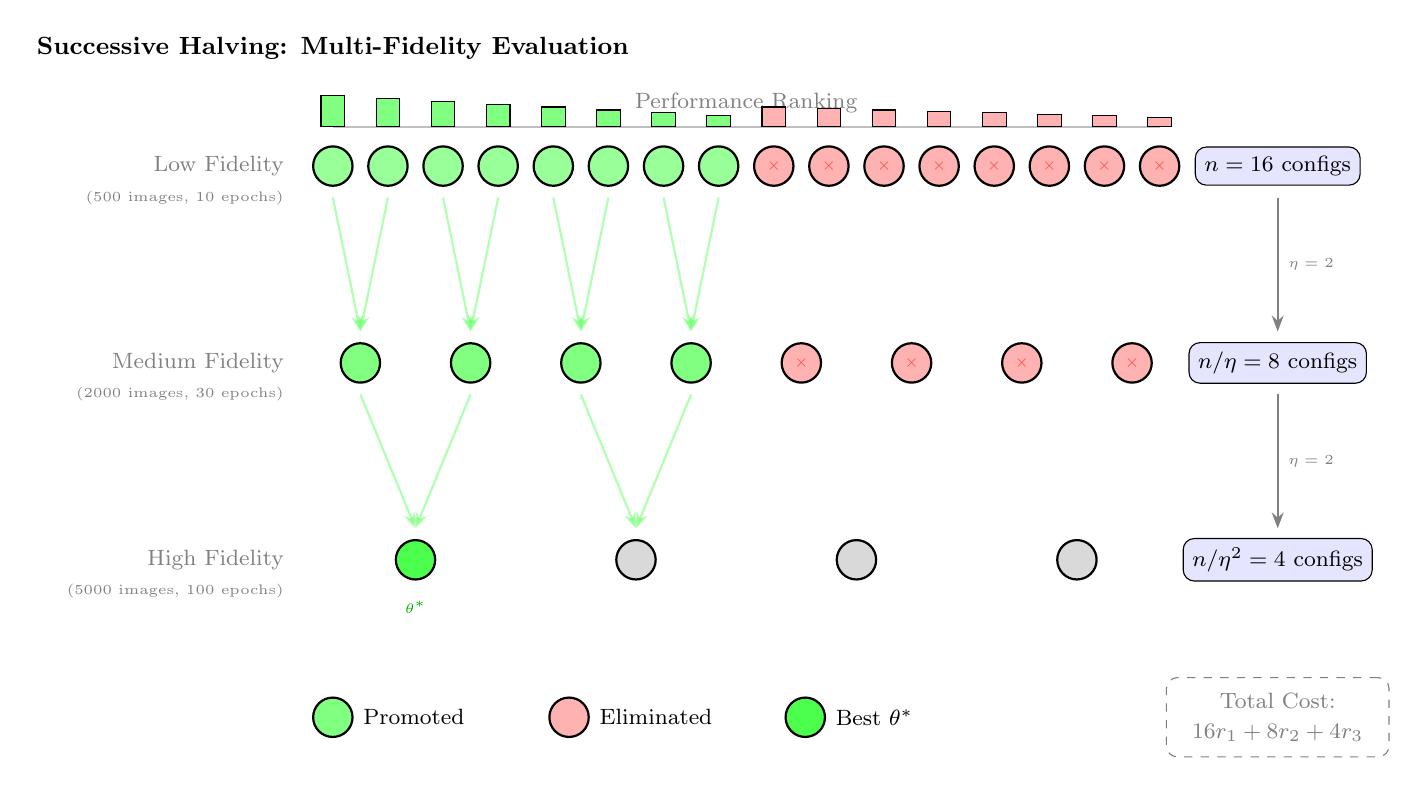
\begin{tikzpicture}[
    node distance=0.6cm,
    every node/.style={font=\small},
    config/.style={circle, draw, thick, minimum size=0.5cm, fill=#1},
    arrow/.style={-{Stealth[length=2mm]}, thick},
    brace/.style={decorate, decoration={brace, amplitude=8pt, raise=3pt, mirror}},
    title/.style={font=\bfseries\small},
    level/.style={font=\footnotesize, gray}
]

% Title
\node[title] at (0, 1.5) {Successive Halving: Multi-Fidelity Evaluation};

% Level labels on left
\node[level, anchor=east] at (-0.5, 0) {Low Fidelity};
\node[font=\tiny, gray, anchor=east] at (-0.5, -0.4) {(500 images, 10 epochs)};

\node[level, anchor=east] at (-0.5, -2.5) {Medium Fidelity};
\node[font=\tiny, gray, anchor=east] at (-0.5, -2.9) {(2000 images, 30 epochs)};

\node[level, anchor=east] at (-0.5, -5) {High Fidelity};
\node[font=\tiny, gray, anchor=east] at (-0.5, -5.4) {(5000 images, 100 epochs)};

% Level 1: Many configurations (16 circles)
\foreach \i in {0,...,15} {
    \pgfmathsetmacro{\xpos}{\i * 0.7}
    \pgfmathsetmacro{\performance}{rnd}
    \ifnum\i<8
        \node[config=green!40] (l1c\i) at (\xpos, 0) {};
    \else
        \node[config=red!30] (l1c\i) at (\xpos, 0) {};
    \fi
}

% X marks for eliminated
\foreach \i in {8,...,15} {
    \pgfmathsetmacro{\xpos}{\i * 0.7}
    \node[font=\tiny, red!70] at (\xpos, 0) {$\times$};
}

% Level 2: 8 configurations
\foreach \i in {0,...,7} {
    \pgfmathsetmacro{\xpos}{\i * 1.4 + 0.35}
    \ifnum\i<4
        \node[config=green!50] (l2c\i) at (\xpos, -2.5) {};
    \else
        \node[config=red!30] (l2c\i) at (\xpos, -2.5) {};
    \fi
}

% X marks for eliminated
\foreach \i in {4,...,7} {
    \pgfmathsetmacro{\xpos}{\i * 1.4 + 0.35}
    \node[font=\tiny, red!70] at (\xpos, -2.5) {$\times$};
}

% Level 3: 4 configurations
\foreach \i in {0,...,3} {
    \pgfmathsetmacro{\xpos}{\i * 2.8 + 1.05}
    \ifnum\i<1
        \node[config=green!70, thick] (l3c\i) at (\xpos, -5) {};
        \node[font=\tiny, green!70!black] at (\xpos, -5.6) {$\theta^*$};
    \else
        \node[config=gray!30] (l3c\i) at (\xpos, -5) {};
    \fi
}

% Arrows connecting levels (showing promotions)
\draw[arrow, green!60, opacity=0.5] (0, -0.4) -- (0.35, -2.1);
\draw[arrow, green!60, opacity=0.5] (0.7, -0.4) -- (0.35, -2.1);
\draw[arrow, green!60, opacity=0.5] (1.4, -0.4) -- (1.75, -2.1);
\draw[arrow, green!60, opacity=0.5] (2.1, -0.4) -- (1.75, -2.1);
\draw[arrow, green!60, opacity=0.5] (2.8, -0.4) -- (3.15, -2.1);
\draw[arrow, green!60, opacity=0.5] (3.5, -0.4) -- (3.15, -2.1);
\draw[arrow, green!60, opacity=0.5] (4.2, -0.4) -- (4.55, -2.1);
\draw[arrow, green!60, opacity=0.5] (4.9, -0.4) -- (4.55, -2.1);

\draw[arrow, green!60, opacity=0.5] (0.35, -2.9) -- (1.05, -4.6);
\draw[arrow, green!60, opacity=0.5] (1.75, -2.9) -- (1.05, -4.6);
\draw[arrow, green!60, opacity=0.5] (3.15, -2.9) -- (3.85, -4.6);
\draw[arrow, green!60, opacity=0.5] (4.55, -2.9) -- (3.85, -4.6);

% Reduction factor annotation
\node[draw, rounded corners, fill=blue!10, font=\footnotesize] at (12, 0) {$n=16$ configs};
\node[draw, rounded corners, fill=blue!10, font=\footnotesize] at (12, -2.5) {$n/\eta = 8$ configs};
\node[draw, rounded corners, fill=blue!10, font=\footnotesize] at (12, -5) {$n/\eta^2 = 4$ configs};

% Arrows showing reduction
\draw[arrow, gray] (12, -0.4) -- node[right, font=\tiny] {$\eta=2$} (12, -2.1);
\draw[arrow, gray] (12, -2.9) -- node[right, font=\tiny] {$\eta=2$} (12, -4.6);

% Cost annotation
\node[draw, dashed, rounded corners, gray, minimum width=2.5cm] at (12, -7) {
    \begin{tabular}{c}
    \footnotesize Total Cost:\\
    \footnotesize $16r_1 + 8r_2 + 4r_3$
    \end{tabular}
};

% Legend
\node[config=green!50, label=right:{\footnotesize Promoted}] at (0, -7) {};
\node[config=red!30, label=right:{\footnotesize Eliminated}] at (3, -7) {};
\node[config=green!70, thick, label=right:{\footnotesize Best $\theta^*$}] at (6, -7) {};

% Performance bar illustration
\node[font=\footnotesize, gray] at (5.25, 0.8) {Performance Ranking};
\draw[thick, gray!50] (0, 0.5) -- (10.5, 0.5);
\foreach \i in {0,...,7} {
    \pgfmathsetmacro{\xpos}{\i * 0.7}
    \pgfmathsetmacro{\height}{0.1 + 0.3 * (8-\i)/8}
    \draw[fill=green!50] (\xpos-0.15, 0.5) rectangle (\xpos+0.15, 0.5+\height);
}
\foreach \i in {8,...,15} {
    \pgfmathsetmacro{\xpos}{\i * 0.7}
    \pgfmathsetmacro{\height}{0.1 + 0.3 * (16-\i)/16}
    \draw[fill=red!30] (\xpos-0.15, 0.5) rectangle (\xpos+0.15, 0.5+\height);
}

\end{tikzpicture}
\end{document}
